RBAC is one of the most efficient models of access control policies~\cite{AhHu2007}.  Began in 1970s with multi-user and multi-application, and has rapidly evolved in the last three decades as a technology for applying a high level security in large-scale systems.  The pivotal idea behind RBAC model is that permissions are associated with roles, and users are administratively assigned to proper roles~\cite{Zha2008}. This mechanism ensures that only authorized users can perform some functions on some data/resources~\cite{FeKu2009}. Generally, RBAC model consists of some basic elements, such as Users, Roles, Permissions, User Assignment (UA), Permissions Assignment (PA) and Constraints (see Figure 1).

\begin{figure}[bht]
\centering
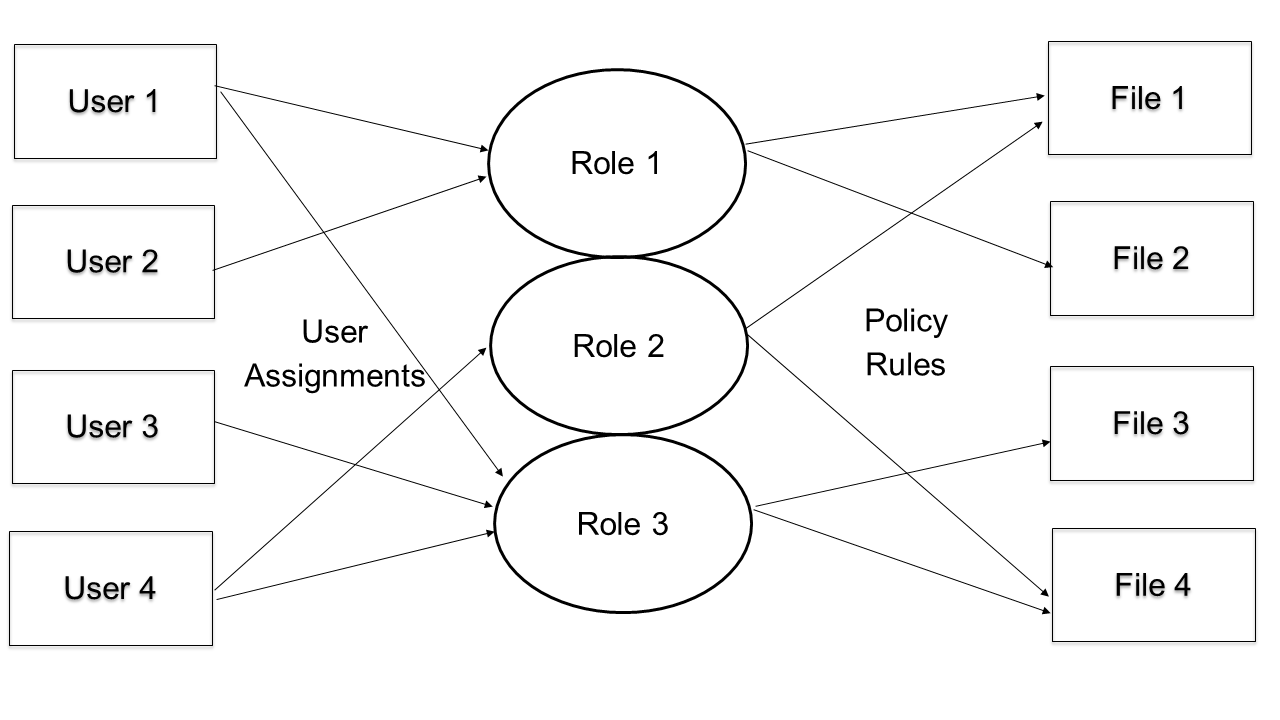
\includegraphics[scale=0.26]{RBACpolicy.png}
\caption{The concept of RBAC security policy.}
\label{fig:RBACPol}
\end{figure}


It is clear that users are not mapped directly into permissions of accessing some resources, but to specific roles which have to be previously assigned to those permissions~\cite{YuBr2012}.  For example, in medical systems, nurses are authorized to access specific resources (e.g. files) which certainly differ from those in which physicians are allowed to.  Therefore, each role in the system (i.e. nurse and physician) is being mapped into the corresponding permissions.  If Alice, for instance, is a nurse, then she has to be assigned to the role $nurse$~\cite{DBS2004}. 
      In RBAC model, there are some relevant terms and concepts, which define the different model's elements~\cite{SDAG2008} (see Figure 2).  However, not all of them are necessary to represent an RBAC security policy, where there are some models that describe only certain needs for a particular system.

\begin{figure}[bht]
\centering
\includegraphics[scale=0.25]{RBACelements.png}
\caption{Elements of RBAC security policy.}
\label{fig:elelmRBAC}
\end{figure}



Table \ref{tab:elements} provides descriptions for the different elements in RBAC models.

\begin{table*}[bth]
\centering
\caption{Description of RBAC's elements.}
\small
\rowcolors{0}{}{lightblue}
\begin{tabular}{p{1.6 in} p{5.2 in}} \hline 
\hline
Code & Description\\\hline

Users (U)&  persons who interact with a system.\\
Roles (R)& prescribed behaviours, which describe particular positions or functions within an organization. \\
Permissions (P)& descriptions of the type of interactions that a user can have with an object.\\
Object& a passive entity that has some information, and   can receive new information.\\
User Assignment (UA)&a many-to-many relationship between users and roles.\\
Permission Assignment (PA)& a many-to-many relationship between permissions and roles.\\
Session (S)& a mapping between a user and any activated role/s that the user is assigned to.\\
Role Hierarchy (RH)& a partial order relationship on roles.\\
Constraints&restrictions on any of the above relationships/assignments.  \\ \hline\hline

\end{tabular}
\label{tab:elements}


\end{table*}


